\hthree{Containersicherheit}

Unter dem Überbegriff "Containersicherheit", wird der Schutz eines Container in einem System verstanden und hierbei die Abwicklung eines Prozesses, eines Services, oder aber auch die gesamte Systeminfrastruktur des Services. \cite{ContainerSecurity}

\begin{figure}[H]
    \centering
    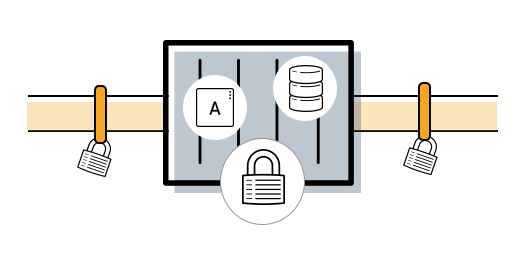
\includegraphics[width=\textwidth]{media/DockerAndContainering/Containersicherheit.png}
    \caption{Containersicherheit \cite{ContainerSecurity}}
\end{figure}

\hfour{Imagesicherheit}

Container oder besser gesagt Services, welche in Containern laufen gelassen werden, werden über sogenannte "Images" bereitgestellt. Dies bietet die Möglichkeit, direkt über ein schädliches "Image" Schadsoftware oder Sicherheitslücken direkt beim Initialisieren des Systems mitzuinstallieren, oder zu öffnen. Wichtig ist daher, dass das "Basisimage", also der Ausgangspunkt für weitere "Images" und Services sicher und geschützt ist. \cite{ContainerSecurity}

Es ist daher wichtig, dass die Entwickler*innen nur "Images" verwenden, welche vertrauenswürdig und sicher sind. Eine 100\% Sicherheit kann jedoch nie gewährleistet sein, da durch das Verändern der Konfiguration oder dem Hinzufügen von neuen Anwendungen wieder Sicherheitslücken entstehen können. \cite{ContainerSecurity}

Ein sicherer Ort für das Auswählen und Verwenden von "Images" ist der "Docker Hub", da im Menü auf der rechten Seite ausgewählt werden kann, ob der Ersteller des "Images" ein verifizierter Ersteller sein muss. \cite{ContainerSecurity}

\begin{figure}[H]
    \centering
    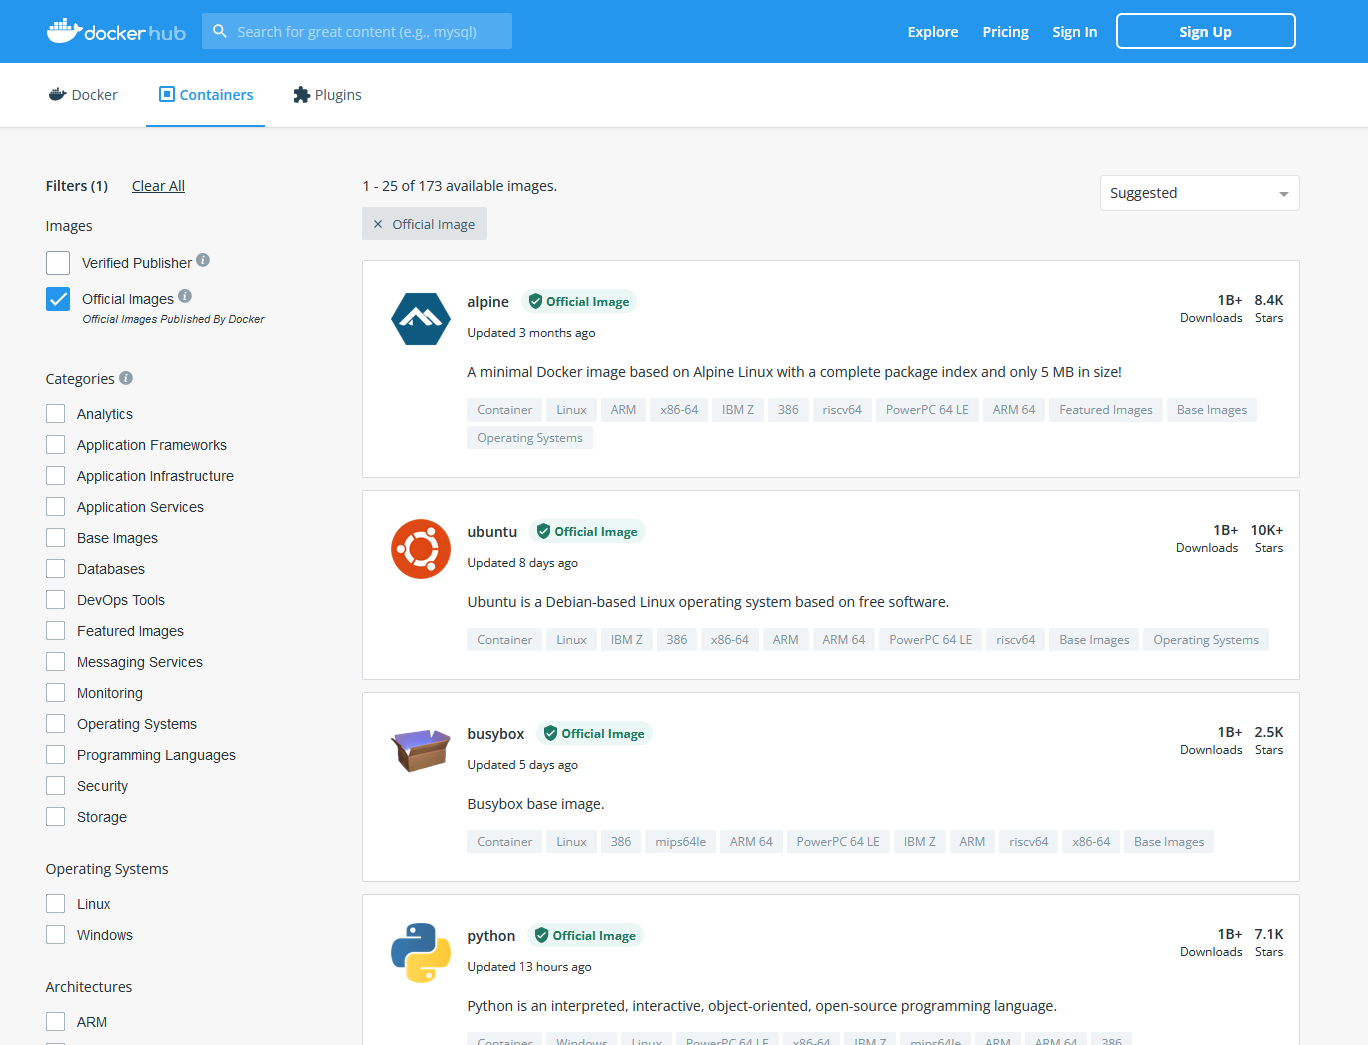
\includegraphics[width=\textwidth]{media/DockerAndContainering/DockerHub.png}
    \caption{"Docker Hub" \cite{DockerHub}}
\end{figure}

Zusammengefasst kann gesagt werden, dass sich vor der Auswahl eines "Images" die Entwickler*innen folgende Fragen stellen sollten:

\begin{itemize}
    \item "Sind diese Images signiert bzw. stammen Sie aus vertrauenswürdigen Quellen?" \cite{ContainerSecurity}
    \item "Sind Runtime- und Betriebssystemschichten aktuell?" \cite{ContainerSecurity}
    \item "Wie schnell und häufig werden die Container aktualisiert?" \cite{ContainerSecurity}
    \item "Wird auf bekannte Probleme überwacht, und wann ja, wie?" \cite{ContainerSecurity}
\end{itemize}

\hfour{Zugriffsverwaltung}

Nachdem der Container nun mit dem gewünschten "Image" richtig aufgesetzt wurde, ist es nun wichtig den Zugriff auf diesen abzusichern. Egal ob der Container nun entwickelt wird (zum Beispiel ein Datenbankcontainer) oder einen Service (beispielsweise einen Service zum Herunterladen) bereitstellt. 

Der Zugriff auf den Container kann durch eine sogenannte "Private Registry" rollenbasiert geregelt werden. Über "Metadaten" kann die Kontrolle von den Daten, auf welche zugegriffen werden soll, kontrolliert werden. Bei "Metadaten" werden beispielsweise schon bekannte Sicherheitslücken weiterverfolgt, oder nach neu auftretenden gesucht. Durch "Private Registry" werden globale Richtlinien für Container und deren "Images" automatisch bereitgestellt. Dies hat den Vorteil, dass menschliches Versagen im Bereich der Richtlinien minimiert werden kann. \cite{ContainerSecurity}

Die Entwickler*innen sollten sich im Bereich der Zugriffsverwaltung Antworten zu folgende vier Fragen überlegen:

\begin{itemize}
    \item "Welche rollenbasierten Kontrollen können Sie für das Management von Container Images nutzen?" \cite{ContainerSecurity}
    \item "Stehen Tagging- oder Kennzeichnungsfunktionen zur Unterstützung der Image-Sortierung zur Verfügung? Können Sie Images separat für Entwicklung, Prüfung und Produktion als genehmigt kennzeichnen?" \cite{ContainerSecurity}
    \item "Bietet die Registry sichtbare Metadaten, mit denen Sie auf bekannte Schwachstellen überwachen können?" \cite{ContainerSecurity}
    \item "Lässt sie sich zur Zuweisung und Automatisierung von Richtlinien (z. B. Prüfung von Signaturen, Codierung von Scans etc.) einsetzen?" \cite{ContainerSecurity}
\end{itemize}

\hfour{Deployment}

Im folgenden Schritt geht es nun darum, das fertige Endservice fortlaufend auf Sicherheitslücken zu prüfen. Sollte eine Lücke entdeckt worden sein, kann diese entweder durch einen "Patch" oder einen "Rebuild" geschlossen werden. "Patches" werden eher nicht gemacht. Es werden eher anhand automatischer Prüfungen Lücken entdeckt und durch automatische Updates und einen "Rebuild" geschlossen. Außerdem bleibt das komplette Neuaufsetzen eines Containers inklusive des Services. \cite{ContainerSecurity}

Bei der Sicherheit im Deploymentbereich sollten die Entwickler*innen folgende Frage beantworten:

\begin{itemize}
    \item "Wie können Sie das Patching ausgeführter Container vermeiden und sie stattdessen per Trigger mithilfe automatischer Updates neu erstellen bzw. ersetzen?" \cite{ContainerSecurity}
\end{itemize}

\cite{ContainerSecurity}

\hfour{Infrastruktur}

Um in diesem Bereich Sicherheit zu bekommen sind die Entwickler*innen auf das Betriebssystem der Hostmaschine angewiesen. Es ist wichtig, dass das Betriebssystem eine hohe Isolierung zwischen den einzelnen Containern bietet und damit Sicherheit bringt. Jedoch kann über "Netzwerk-Namespaces" beispielsweise eine gemeinsame Nutzung von Speicher zwischen den Containern ermöglicht werden. Es sollte aber jede Anwendung auch die nötigen Sicherheitsvorkehrungen (Authentifizierung, Autorisierung, Durchsatzbeschränkungen, usw.) implementiert haben, um sich nicht rein auf die Containersicherheit oder die Infrastruktursicherheit zu verlassen. \cite{ContainerSecurity}

Die Entwickler*innen sollten sich aber im Bereich der Infrastruktursicherheit bei der Implementierung folgende Fragen stellen:

\begin{itemize}
    \item "Welche Container müssen aufeinander zugreifen können? Wie können sich Container gegenseitig ermitteln?" \cite{ContainerSecurity}
    \item "Wie sollen der Zugriff auf und das Management von gemeinsamen Ressourcen (\zb\ Netzwerk und Storage) kontrolliert werden?" \cite{ContainerSecurity}
    \item "Wie werden Host-Updates verwaltet? Müssen all Ihre Container gleichzeitig aktualisiert werden?" \cite{ContainerSecurity}
    \item "Wie überwachen Sie den Container-Zustand?" \cite{ContainerSecurity}
\end{itemize}
